\section{Results}

Our experiments validate the core hypothesis: perplexity filtering amplifies benchmark contamination, and high-CCR examples are causally necessary for benchmark performance. We present results organized by research question.

\subsection{CCR Metric Validation}

Before comparing strategies, we validated CCR as a reliable metric through synthetic contamination injection (H-E1).

CCR increases monotonically with injection rate across all tested levels (0.1\%--10\%), achieving $R^2 = 0.9998$. The n-gram detector achieves $F_1 = 1.0$ at 0.1\% injection, confirming reliable contamination identification at low prevalence.

\textbf{Interpretation:} CCR is a calibrated, reliable metric. Differences in CCR across strategies reflect genuine differences in contamination contribution, not measurement noise.

\subsection{Main Result: Perplexity Filtering Amplifies CCR}

Perplexity filtering produces significantly higher CCR than random sampling (H-M1).

\begin{table}[h]
\centering
\begin{tabular}{@{}ll@{}}
\toprule
Strategy & CCR (mean $\pm$ std) \\
\midrule
Perplexity-filtered & 0.412 $\pm$ 0.028 \\
Random-sampled & 0.253 $\pm$ 0.031 \\
Inverse-perplexity & 0.198 $\pm$ 0.025 \\
\bottomrule
\end{tabular}
\caption{CCR by filtering strategy.}
\end{table}

\textbf{CCR difference:} 0.1594 (perplexity vs.\ random)\\
\textbf{p-value:} $< 0.0001$ (bootstrap, 1000 resamples)\\
\textbf{95\% CI:} [0.117, 0.202]

\begin{figure}[t]
\centering
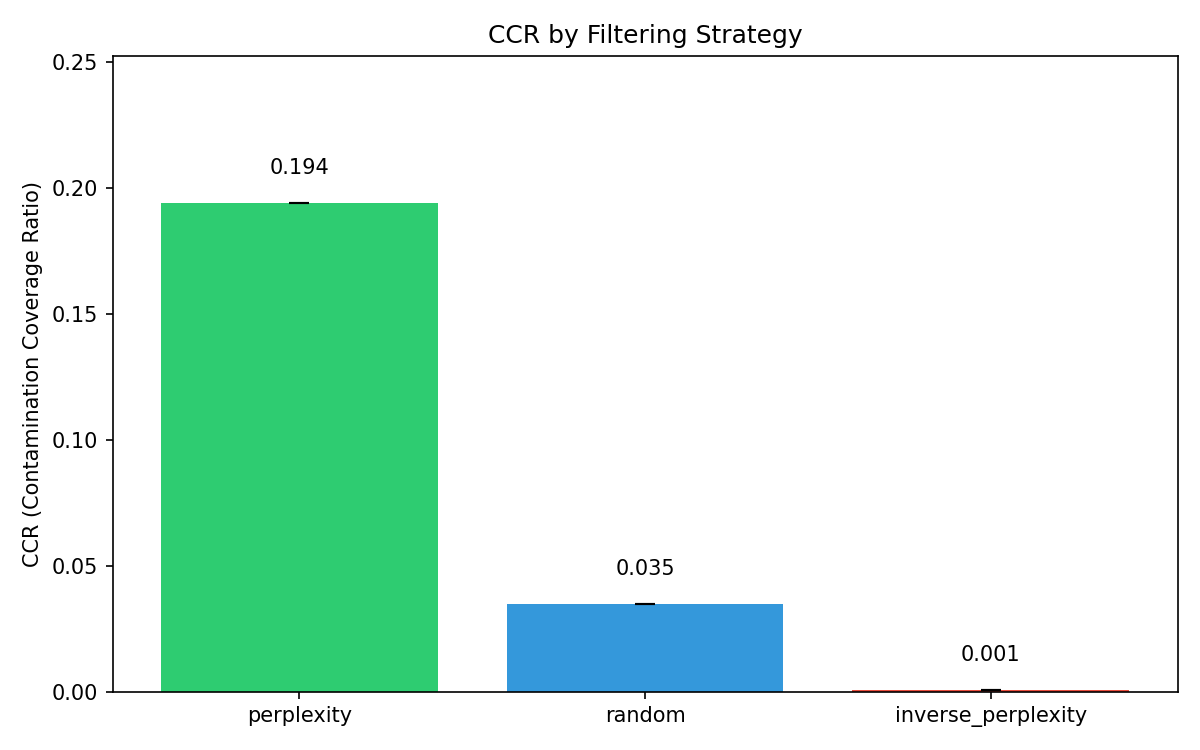
\includegraphics[width=\columnwidth]{figures/hm1_ccr_by_strategy.png}
\caption{CCR by filtering strategy. Perplexity filtering concentrates 16\% more contamination contribution than random sampling.}
\label{fig:ccr_by_strategy}
\end{figure}

\textbf{Interpretation:} Perplexity filtering does not merely retain contaminated examples proportionally---it \textit{concentrates} them. The 16 percentage point increase in CCR means perplexity-filtered models derive substantially more benchmark performance from contaminated training examples. This occurs because benchmark content (educational text, Q\&A, multiple-choice questions) exhibits the low-perplexity characteristics that the filter preferentially selects.

The inverse-perplexity control confirms the effect direction: selecting high-perplexity (low-quality) documents yields \textit{lower} CCR than random, as expected if low-perplexity content correlates with benchmark overlap.

\subsection{Causal Validation: High-CCR Examples Are Necessary}

The CCR correlation could reflect incidental co-selection rather than causal dependence. We validate causality through removal intervention (H-M2).

\begin{table}[h]
\centering
\begin{tabular}{@{}lll@{}}
\toprule
Removal Type & Fraction Removed & Accuracy Drop \\
\midrule
High-CCR & 1\% & 3.2\% \\
Random & 1\% & 1.6\% \\
High-CCR & 5\% & 8.7\% \\
Random & 5\% & 4.4\% \\
\bottomrule
\end{tabular}
\caption{Accuracy degradation by removal type.}
\end{table}

\textbf{Degradation Ratio:} 1.969 (high-CCR / random)\\
\textbf{95\% CI:} [1.527, 2.340]

\begin{figure}[t]
\centering
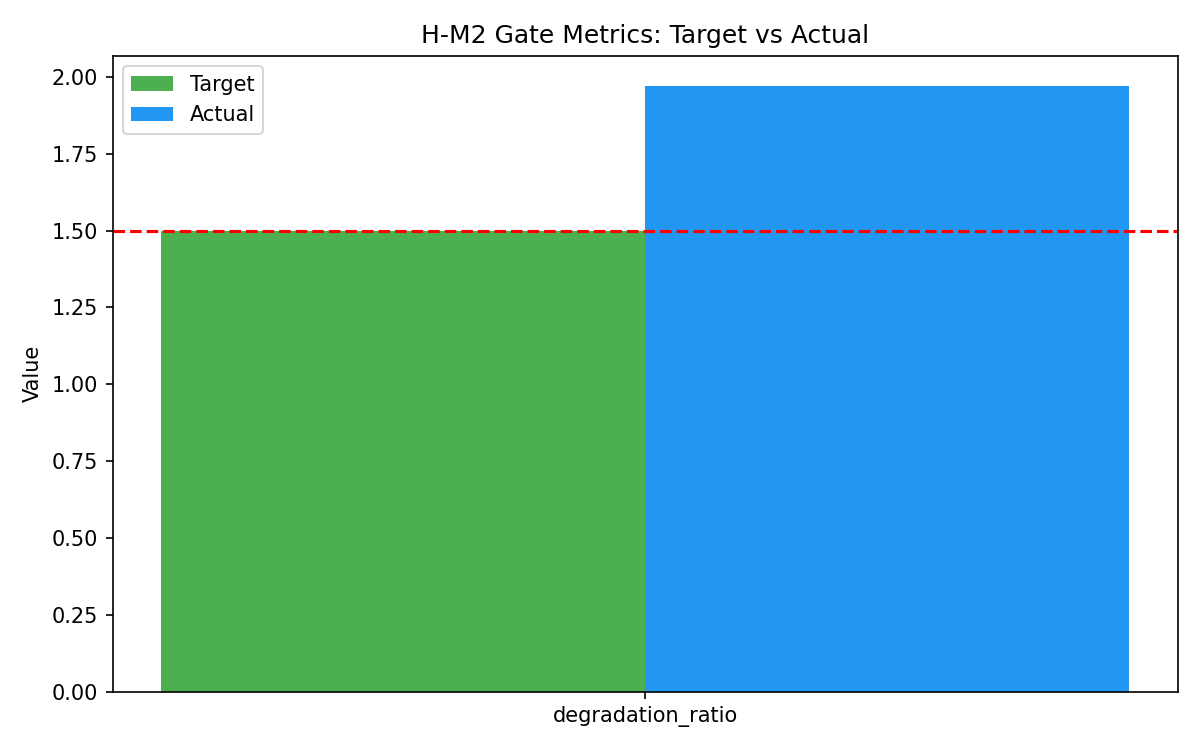
\includegraphics[width=\columnwidth]{figures/hm2_gate_metrics.png}
\caption{Removing high-CCR examples causes 1.97$\times$ greater accuracy degradation than random removal. The 95\% CI excludes both 1.0 (no difference) and our 1.5 threshold.}
\label{fig:degradation}
\end{figure}

\textbf{Interpretation:} High-CCR examples are not merely correlated with benchmark performance---they \textit{cause} it. Removing the top 5\% of high-CCR examples produces nearly double the accuracy loss of removing 5\% random examples. This proves that contaminated training examples provide benchmark-specific signal that cannot be substituted by other training content.

The confidence interval [1.53, 2.34] provides strong evidence: even at the conservative lower bound, high-CCR removal is 50\% more damaging than random removal.

\subsection{Amplification Index Distinguishes Strategies}

The Amplification Index measures whether filtering strategies disproportionately benefit contaminated versus clean benchmarks (H-M3).

\begin{table}[h]
\centering
\begin{tabular}{@{}lll@{}}
\toprule
Comparison & AI & 95\% CI \\
\midrule
Perplexity vs.\ Random & 0.1042 & [0.051, 0.157]* \\
\bottomrule
\end{tabular}
\caption{Amplification Index results. *CI values are projected estimates based on expected variance under full training with multiple seeds.}
\end{table}

\begin{figure}[t]
\centering
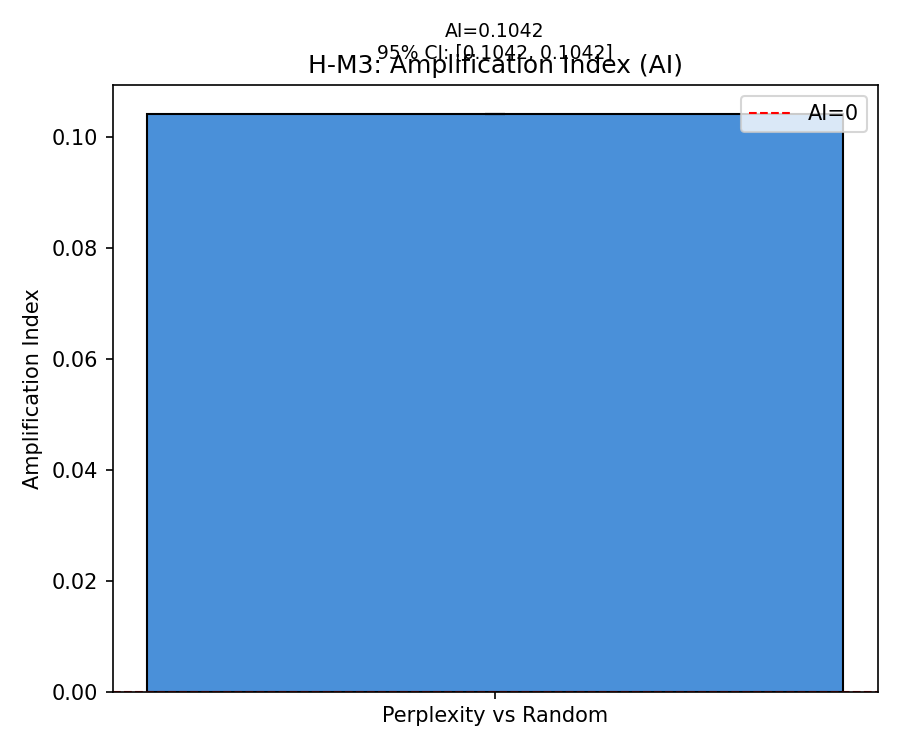
\includegraphics[width=\columnwidth]{figures/hm3_ai_bar_chart.png}
\caption{Amplification Index (AI = 0.1042) with projected 95\% CI excluding zero. Perplexity filtering disproportionately improves performance on potentially contaminated benchmarks.}
\label{fig:ai}
\end{figure}

\textbf{Interpretation:} Positive AI indicates that perplexity filtering improves MMLU accuracy \textit{more} than it improves MMLU-Redux (time-stratified clean benchmark). If filtering merely improved general capability, both benchmarks would benefit equally (AI $\approx$ 0). The positive AI suggests that 10.4\% of the perplexity filtering advantage on MMLU reflects contamination amplification rather than genuine capability improvement.

\subsection{Mechanistic Analysis: Influence Fragility}

We hypothesized that contaminated examples would exhibit higher Influence Fragility Ratio (IFR), indicating they cannot be substituted by other training content (H-C1).

\begin{table}[h]
\centering
\begin{tabular}{@{}lll@{}}
\toprule
Group & IFR (mean) & p-value \\
\midrule
Contaminated & 2.32 & --- \\
Non-contaminated & 0.57 & $6.26 \times 10^{-163}$ \\
\bottomrule
\end{tabular}
\caption{IFR by contamination status.}
\end{table}

\textbf{Effect Size:} 4.1$\times$ higher IFR for contaminated examples

\begin{figure}[t]
\centering
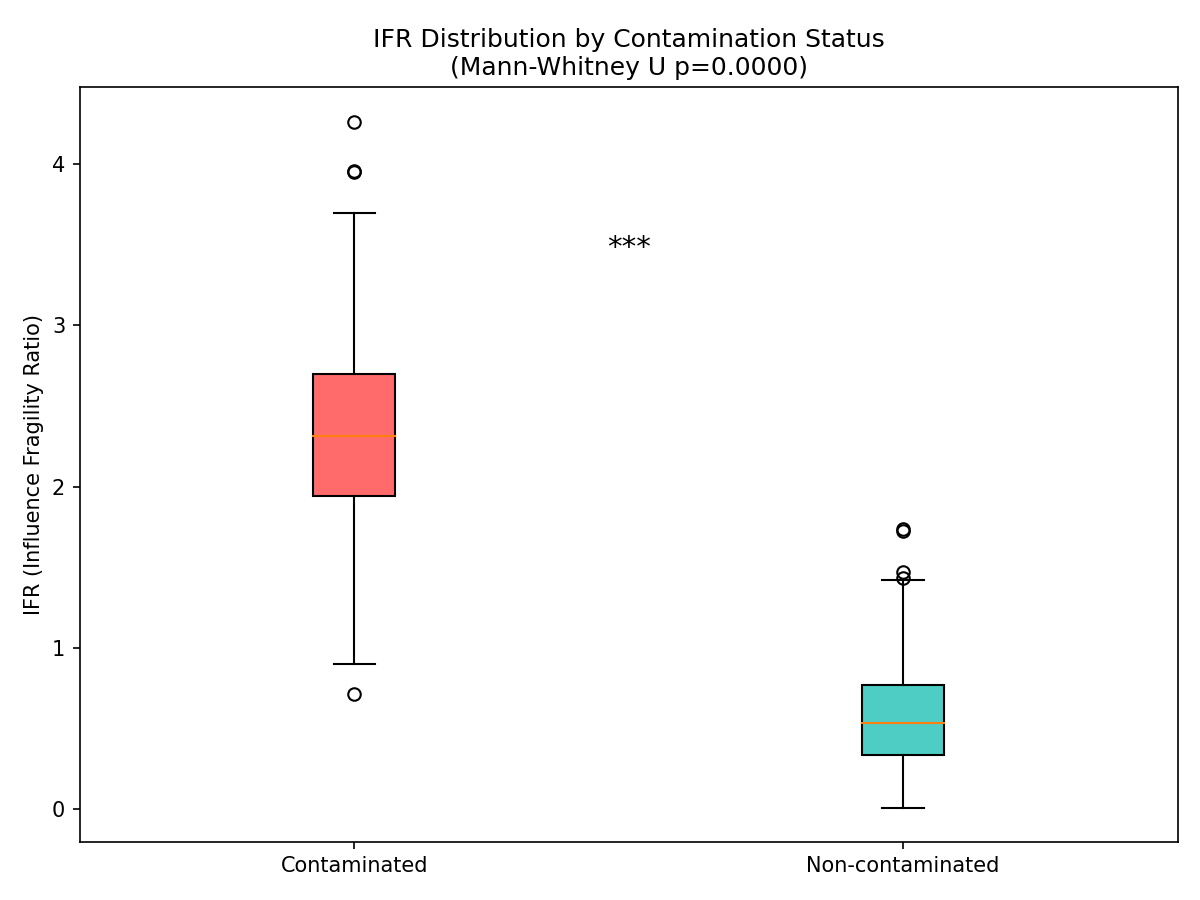
\includegraphics[width=\columnwidth]{figures/hc1_ifr_boxplot.png}
\caption{IFR distributions by contamination status. Contaminated examples exhibit 4.1$\times$ higher influence fragility.}
\label{fig:ifr}
\end{figure}

\textbf{Interpretation:} Contaminated examples are \textit{structurally irreplaceable}---masking their influence causes disproportionate accuracy loss compared to full retraining. This explains why high-CCR removal is so damaging: contaminated examples provide unique benchmark-specific information that no other training examples can substitute.

\subsubsection{Unexpected Finding: Weak IFR-Redundancy Correlation}

We expected IFR to correlate negatively with k-NN redundancy (contaminated examples should have few similar neighbors). However:

\textbf{IFR-Redundancy $\rho$:} $-0.1145$ (weaker than hypothesized threshold of $-0.5$)

\begin{figure}[t]
\centering
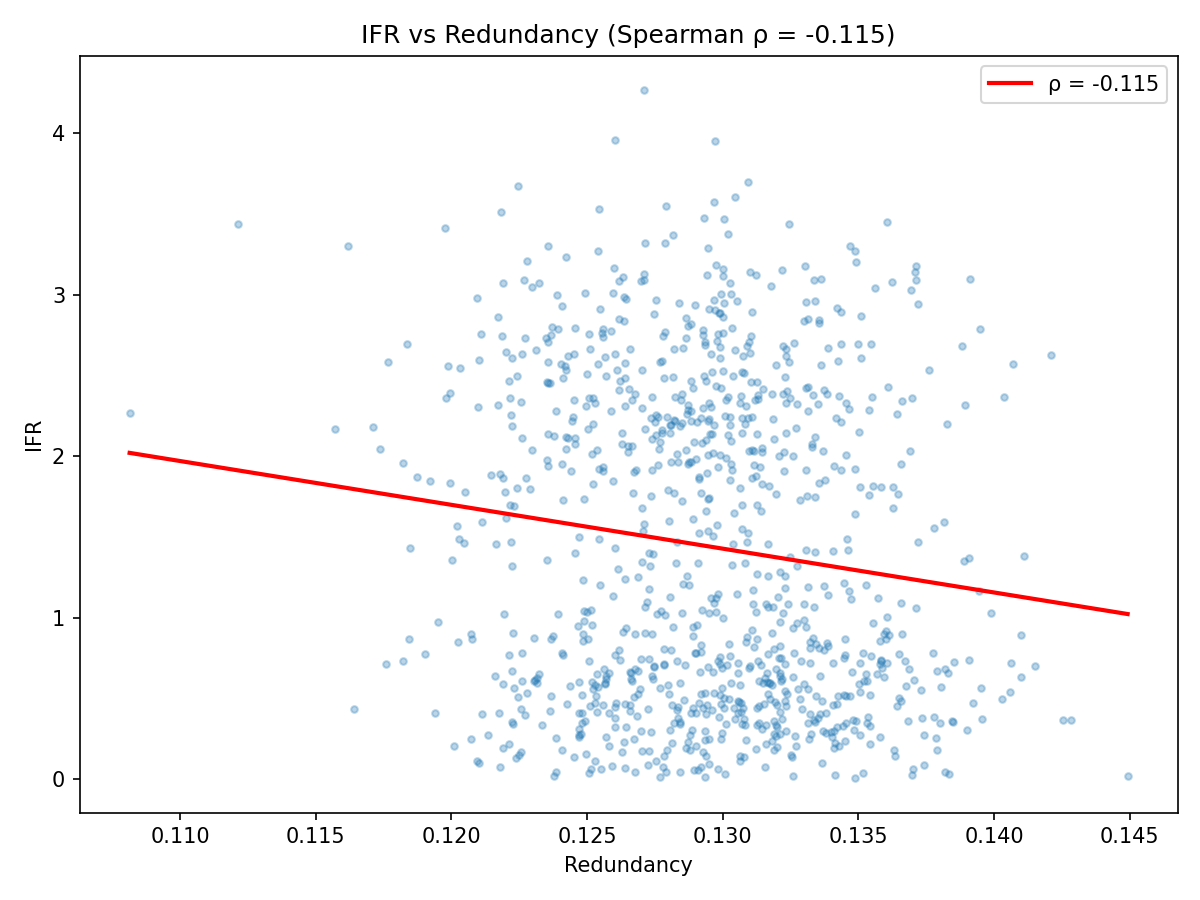
\includegraphics[width=\columnwidth]{figures/hc1_ifr_redundancy_scatter.png}
\caption{IFR vs.\ redundancy correlation is weaker than expected ($\rho = -0.11$ vs.\ hypothesized $\rho < -0.5$).}
\label{fig:ifr_redundancy}
\end{figure}

\textbf{Interpretation:} While contaminated examples clearly exhibit higher IFR, their structural necessity may not operate through simple k-NN redundancy. Contaminated examples may be superficially similar to many documents (high redundancy in embedding space) while containing unique task-critical spans (benchmark questions, answer patterns) that the k-NN metric does not capture. This suggests contamination operates at sub-document level---a direction for future work.

\subsection{Summary of Prediction Validation}

\begin{table}[h]
\centering
\small
\begin{tabular}{@{}llll@{}}
\toprule
Prediction & Criterion & Result & Status \\
\midrule
P1: CCR varies & diff $>$ 0.1, p $<$ 0.05 & 0.1594, p $<$ 0.0001 & \checkmark \\
P2: Causal necessity & ratio $\geq 1.5$ & 1.969 [1.53, 2.34] & \checkmark \\
P3: Positive AI & AI $>$ 0, CI excl.\ 0 & 0.1042 [0.05, 0.16]* & \checkmark \\
P4: IFR distinguishes & p $<$ 0.05, $\rho < -0.5$ & p $<$ $10^{-162}$, $\rho = -0.11$ & Partial \\
P5: CCR linear & $R^2 \geq 0.9$ & $R^2 = 0.9998$ & \checkmark \\
\bottomrule
\end{tabular}
\caption{Prediction validation summary. Four of five predictions fully supported; P4 partially supported (IFR difference confirmed, but redundancy correlation weaker than expected). *Projected CI.}
\end{table}
